\section{Classical Runge-Kutta method with fixed time step size} \label{part5}
We consider again the initial value problem in (\ref{2_problem}).

\subsection{Describe the classical Runge-Kutta method with fixed step size} \label{5_1}

The classical Runge-Kutta is an iterative method used to calculate numerical approximations to the solution of initial value problems. It works by taking a time step size $h$, where we will perform the following calculations:

\begin{align*}
    &T_1 = t_n &&X_1 = x_n \\
    &T_2 = t_n + \frac{1}{2}h  &&X_2 = x_n + h\frac{1}{2}f(T_1, X_1) \\
    &T_3 = t_n + \frac{1}{2}h  &&X_3 = x_n + h\frac{1}{2}f(T_2, X_2) \\
    &T_4 = t_n + h  &&X_4 = x_n + hf(T_3, X_3) \\
\end{align*}
Once this is calculated, we can get the actual step that we will store as part of our solution as follows:
\begin{gather*}
    t_{n+1} = t_n + h \\
    x_{n+1} = x_n + h\left(\frac{1}{6}f(T_1, X_1) + \frac{1}{3}f(T_2,X_2) + \frac{1}{3}f(T_3, X_3) + \frac{1}{6}f(T_4,X_4)\right)
\end{gather*}
Note that the previous 8 calculations must be performed in every single step. To solve the initial value problem we just start from $x_0$, pick a step size $h$, and iterate over the algorithm.

\begin{table}[H]
    \centering
    \begin{tabular}{c|cccc}
    0   &     &     &     &     \\
    $\nicefrac{1}{2}$ & $\nicefrac{1}{2}$ &     &     &     \\
    $\nicefrac{1}{2}$ & 0   & $\nicefrac{1}{2}$ &     &     \\
    $1$   & 0   & 0   & $1$   &     \\ \hline
    x   & $\nicefrac{1}{6}$ & $\nicefrac{1}{3}$ & $\nicefrac{1}{3}$ & $\nicefrac{1}{6}$
    \end{tabular}
    \caption{Butcher Tableau of the classical Runge-Kutta method}
    \label{5_BT_RK4}
\end{table}

%%%%%%%%%%%%%%%%%%%%%%%%%%%%%%%%%%%%%%%%%%%%%%%%%%%%%%%%%%%%%%%%%%%%%%%%%%%%%%%%%%%%%%%%%%%%%%%%%%%

\subsection{Implement an algorithm in Matlab for the classical Runge-Kutta method with fixed time step size. Provide the code in your report.  Use a format that enables syntax highlighting. Comment on the code}
We implement the classical Runge-Kutta method with fixed time step size with the following code:
\begin{lstlisting}[caption = Classical Runge-Kutta method with fixed time step size, captionpos=b, label=1_ClassicRK4]
function [T, X] = ClassicRK4_fixed(fun,tspan,h,x0,args)
% time interval
t0 = tspan(1);
tf = tspan(end);
T = t0:h:tf;
N = size(T,2);
X = zeros(size(x0,1), N);
X(:,1) = x0;

for k = 1:N-1
    t = T(k);
    x = X(:,k);

    % Stage 1
    T1 = t;
    X1 = x;
    F1 = feval(fun,T1,X1,args{:});
    % Stage 2
    T2 = t + h/2;
    X2 = x + h/2*F1;
    F2 = feval(fun,T2,X2,args{:});
    % Stage 3
    T3 = T2;
    X3 = x + h/2*F2;
    F3 = feval(fun,T3,X3,args{:});
    % Stage 4
    T4 = t + h;
    X4 = x + h*F3;
    F4 = feval(fun,T4,X4,args{:});

    % final solution
    X(:,k+1) = x + h*(1/6*F1+1/3*F2+1/3*F3+1/6*F4);

end
end
\end{lstlisting}

This implementation uses the following input arguments:
\begin{itemize}
    \item \code{fun} is a pointer to a function where our IVP function $f$ is defined.
    \item \code{tspan} is a vector of two values stating the initial and final time of the simulation.
    \item \code{x0} is the initial condition, i.e. the value of $x(t_0)$.
    \item \code{h} is the fixed time step size we want for our simulation.
    \item \code{args} is an array that includes constants needed to calculate the IVP function ($\mu$ in the Van der Pol problem, $\lambda$ in the test equation, all the parameters in the CSTR problem).
\end{itemize}


%%%%%%%%%%%%%%%%%%%%%%%%%%%%%%%%%%%%%%%%%%%%%%%%%%%%%%%%%%%%%%%%%%%%%%%%%%%%%%%%%%%%%%%%%%%%%%%%%%%
\subsection{Test your problem for test equation. Discuss order and stability of the numerical method} \label{5_3}
We will proceed testing the classical Runge-Kutta method (RK4) in a similar manner as we did for the Explicit and Implicit Euler methods in part \ref{part1}. As the RK4 has order 4, we should observe the local error having order 5 and the global error having order 4. Results are shown in the folowing figures, setting $\lambda=-1$, $h=0.2$ for \ref{5_3_TE} and $\code{tspan}=[0, 30]$ for \ref{5_3_TE_errors}.

The shape of the local and global errors vs. time is very similar to the one obtained for the Explicit and Implicit Euler in Figure \ref{1_3_errors}. However, both having the same time step size, the solution of the RK4 is a lot more precise. The scale of the errors is not even comparable.

\begin{figure}[H]
    \centering
    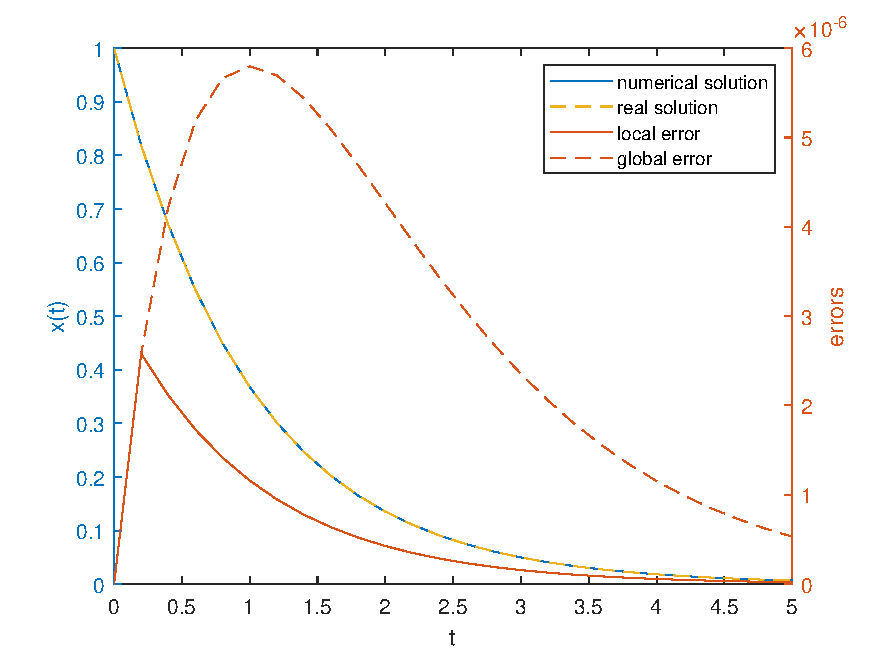
\includegraphics[width=0.7\linewidth]{images/5/5_3_TestEquation.pdf} 
    \caption{Solution and errors vs. time for the Test equation using fixed classical Runge-Kutta method}
    \label{5_3_TE}
\end{figure}

\begin{figure}[H]
\centering
    \begin{subfigure}{0.49\linewidth}
        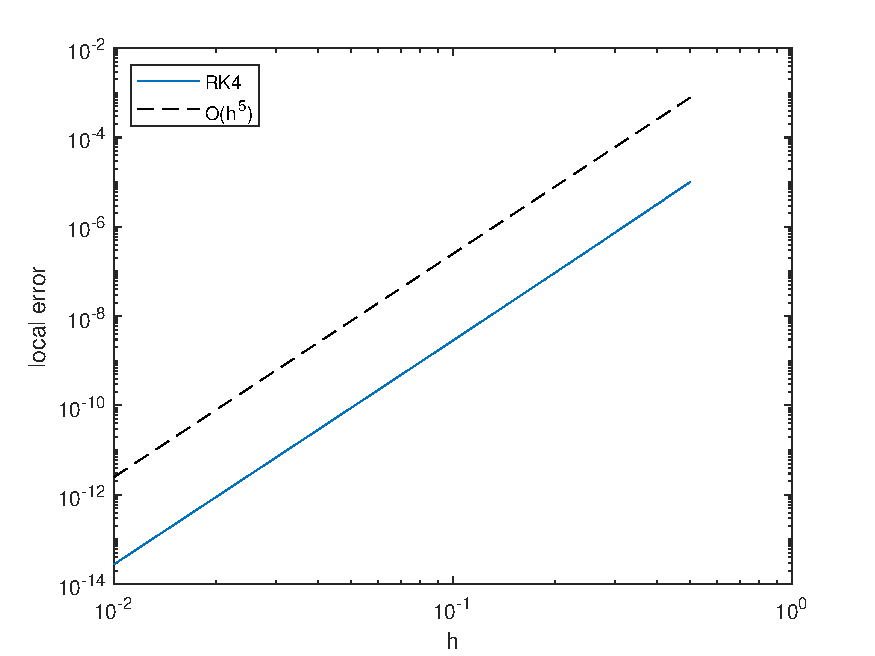
\includegraphics[width=\linewidth]{images/5/5_3_localerror.pdf}
        \caption{Local error}
    \end{subfigure}
    \begin{subfigure}{0.49\linewidth}
        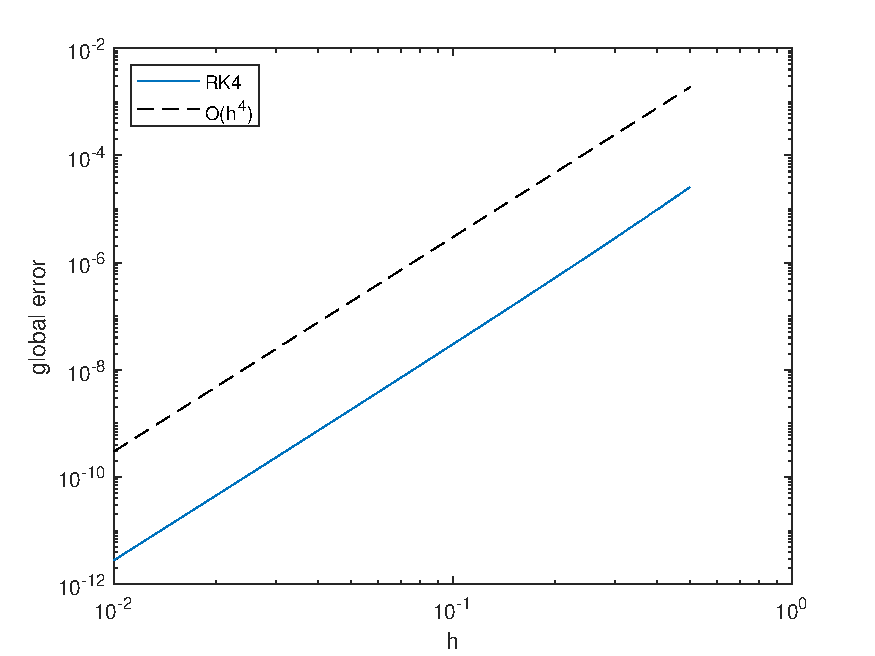
\includegraphics[width=\linewidth]{images/5/5_3_globalerror.pdf}
        \caption{Global error}
    \end{subfigure}
    \caption{Local and global errors vs. time-step size for the Test equation using fixed classical Runge-Kutta method}
    \label{5_3_TE_errors}
\end{figure}

For the stability of the method, the solution by a Runge-Kutta method for the test equation is given as:
\begin{equation} \label{stability_region_formula}
    x_{n+1} = R(h \lambda) x_n \hspace{1em} R(z) = 1 + z b'(I-zA)^(-1)e,
\end{equation}
where, A and b are the top right matrix and the bottom right vector in the Butcher Tableau \ref{5_BT_RK4}. The stability regions for complex values of $h\lambda$ are shown in Figure \ref{5_3_stability_regions}. Here we can observe that the method is neither A-stable, nor L-stable, given that there are regions on the left side plane that are greater than 1 and that $\lim_{z \to -\infty}|R(z)| \neq 0$.

\begin{figure}[H]
    \centering
    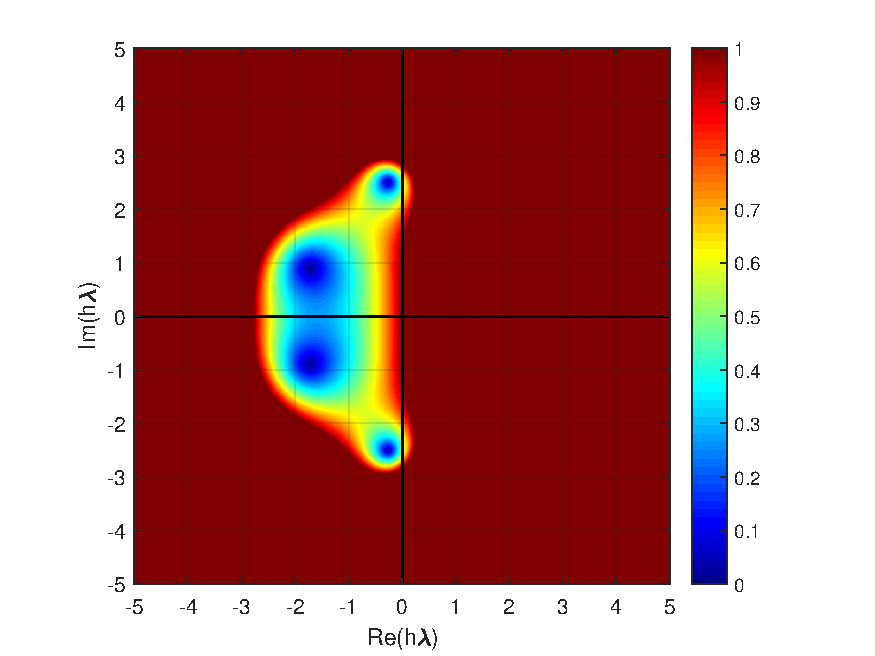
\includegraphics[width=0.7\linewidth]{images/5/5_3_stability_regions.pdf} 
    \caption{Values of $R(h\lambda)$ for the classical Runge-Kutta method}
    \label{5_3_stability_regions}
\end{figure}

%%%%%%%%%%%%%%%%%%%%%%%%%%%%%%%%%%%%%%%%%%%%%%%%%%%%%%%%%%%%%%%%%%%%%%%%%%%%%%%%%%%%%%%%%%%%%%%%%%%

\subsection{Test your algorithms on the Van der Pol problem \texorpdfstring{($\mathbf{\mu = 1.5}$ and $\mathbf{\mu = 15}$, $\mathbf{x_0 = [1.0;1.0]}$).}{(mu = 1.5 and mu = 15, x0 = [1.0;1.0]).}}
We can observe that the classical Runge-Kutta manages to approach the real solution with a way bigger step size than the Explicit Euler (Figures \ref{2_4_fixed_mu_1_5} and \ref{2_4_fixed_mu_15}) in both cases. However, for $\mu=15$ we need to lower the step size almost by a factor of 10 due to the larger stiffness of the problem. After all, the classical Runge-Kutta is a explicit method and thus suffer from the same problems as the Explicit Euler.

\begin{figure}[H]
    \centering
    \makebox[\textwidth][c]{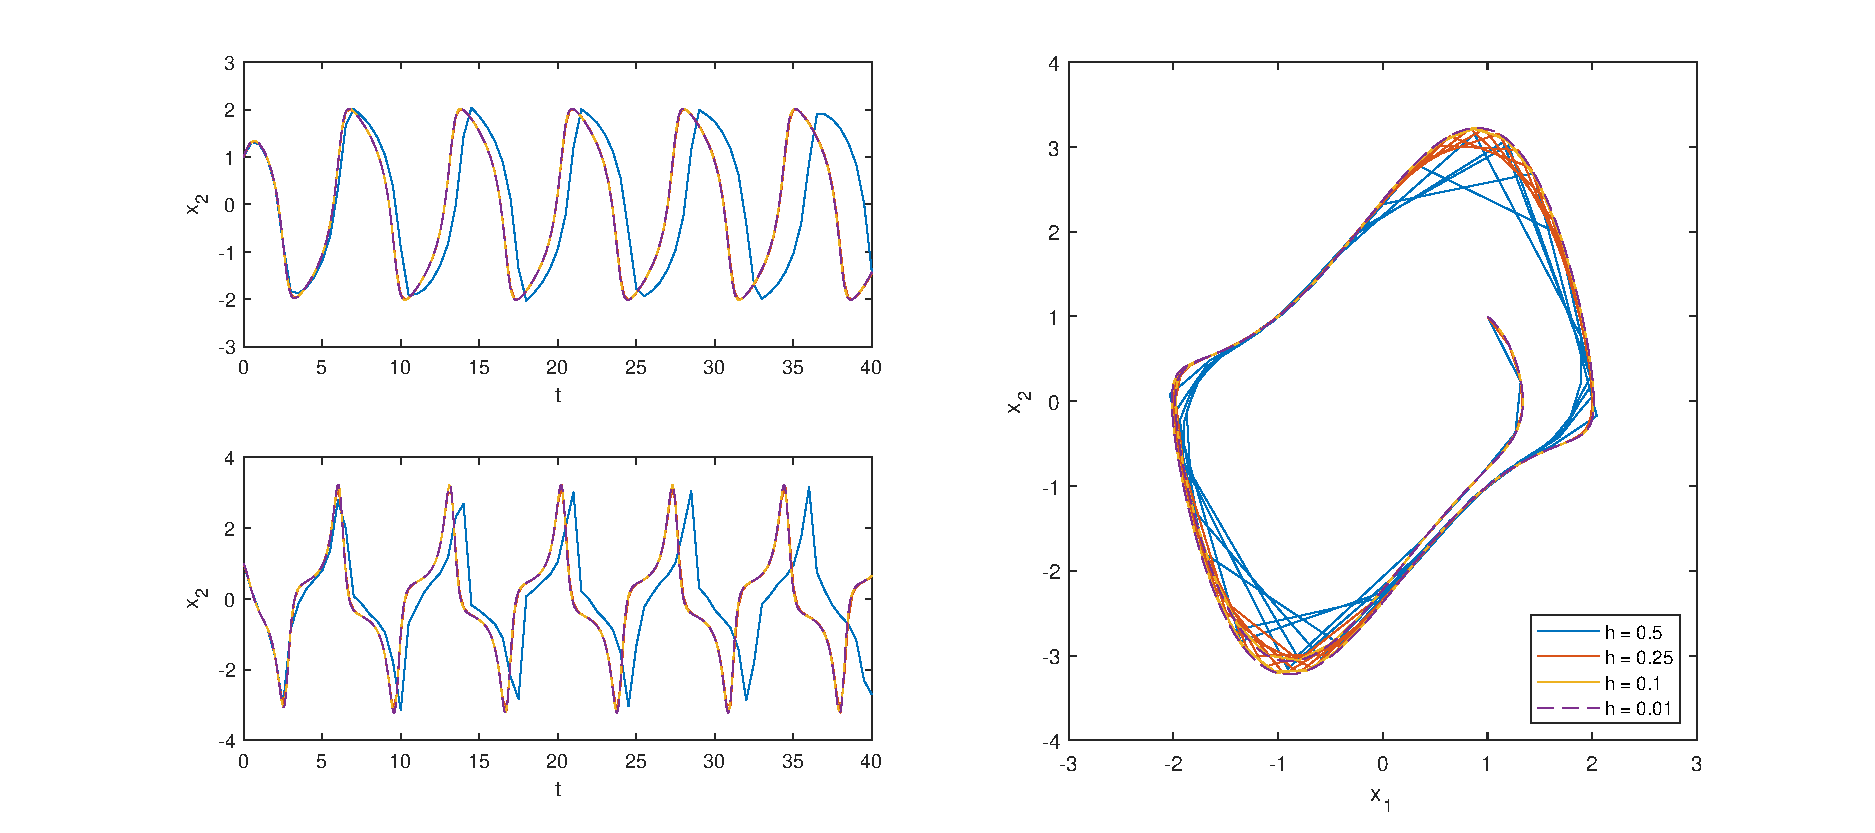
\includegraphics[width=1.25\textwidth]{images/5/5_4_RK4_mu_1_5.pdf}}
    \caption{Solution for the Van der Pol problem ($\mathit{\mu = 1.5}$) using classical Runge-Kutta with fixed step size}
    \label{5_4_RK4_mu_1_5}
\end{figure}

\begin{figure}[H]
    \centering
    \makebox[\textwidth][c]{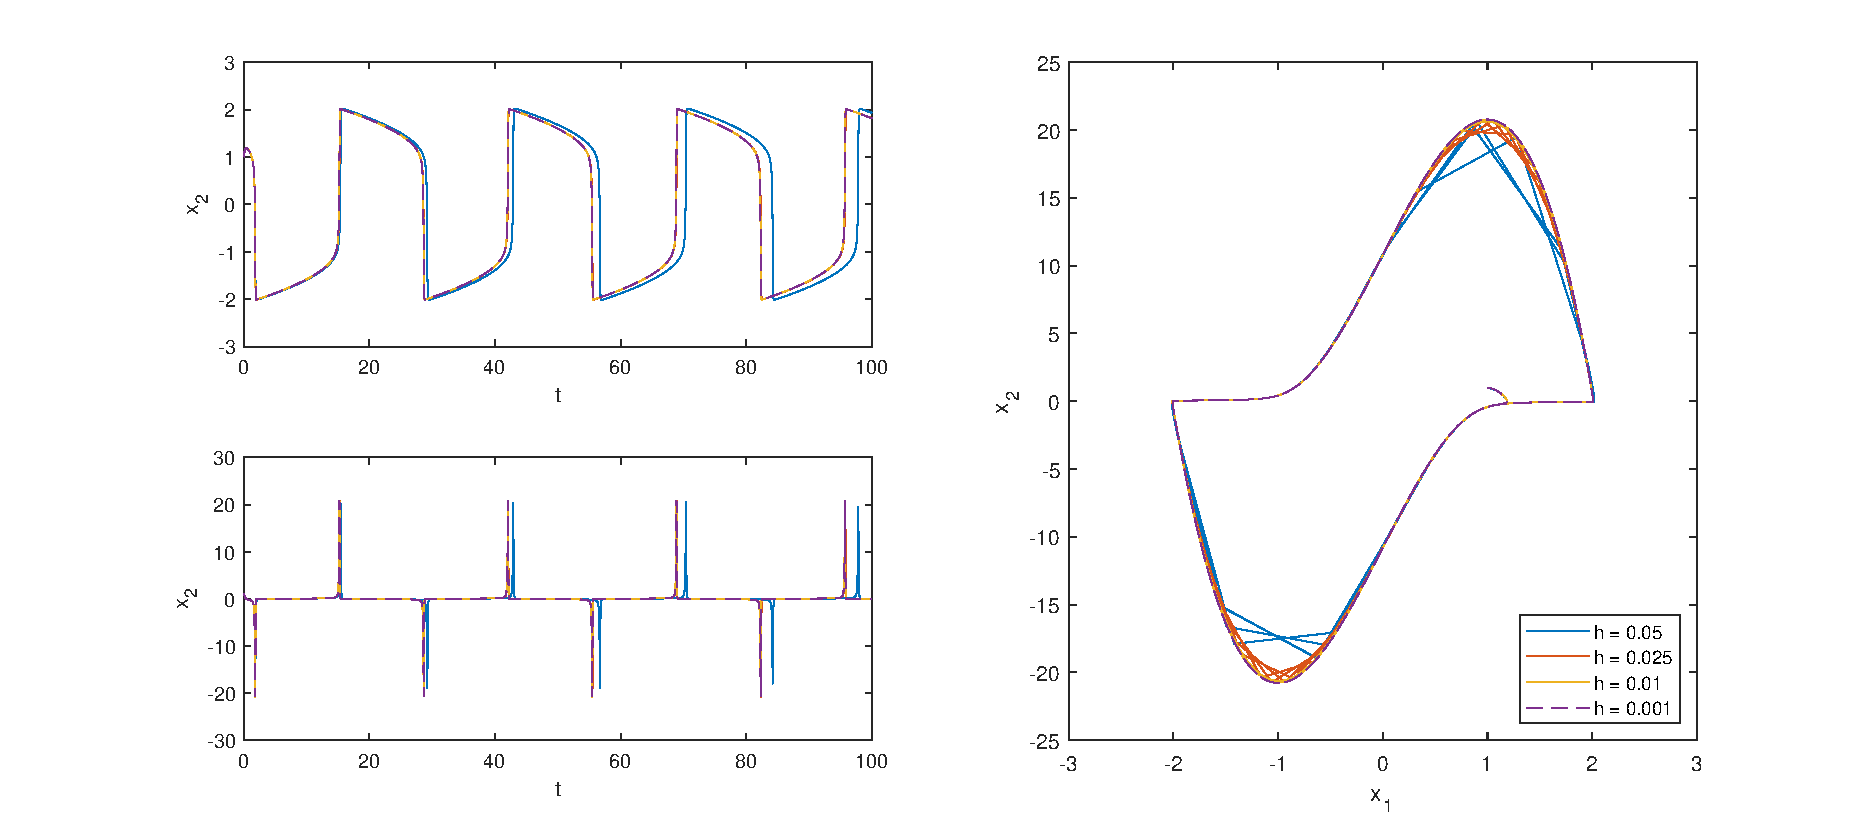
\includegraphics[width=1.25\textwidth]{images/5/5_4_RK4_mu_15.pdf}}
    \caption{Solution for the Van der Pol problem ($\mathit{\mu = 15}$) using classical Runge-Kutta with fixed step size}
    \label{5_4_RK4_mu_15}
\end{figure}


%%%%%%%%%%%%%%%%%%%%%%%%%%%%%%%%%%%%%%%%%%%%%%%%%%%%%%%%%%%%%%%%%%%%%%%%%%%%%%%%%%%%%%%%%%%%%%%%%%%

\subsection{Test  your  algorithms  on  the  adiabatic  CSTR  problem  described  in  the
papers uploaded to Learn (3D-version and 1D-version).}
For the CSTR problem, we can still see an increase in performance compared to the Explicit Euler (Figure \ref{2_5_3D_1D_hs}) but not as significant as in the Van der Pol case. We can still see the spiky behaviour when $T$ reaches its maximum (low $F$), when the problem is more stiff. The step size of $h=0.1$ already approaches the solution pretty good, only failing at some values in this stiff area of the problem.
\begin{figure}[H]
\centering
    \begin{subfigure}{0.8\linewidth}
        \centering
        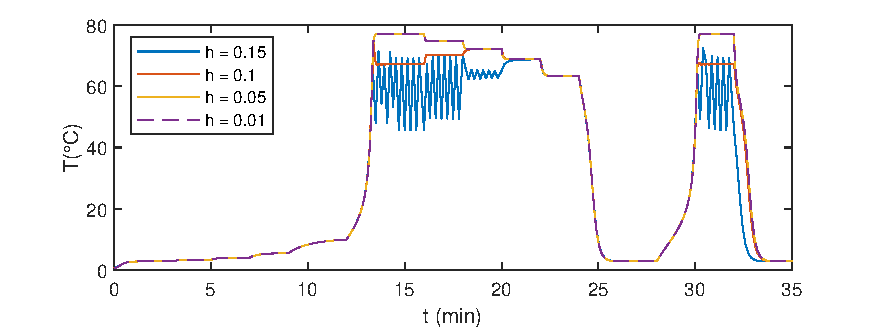
\includegraphics[width=1\linewidth]{images/5/5_5_CSTR_3D.pdf} 
        \caption{CSTR 3D problem}
    \end{subfigure} \\
    \begin{subfigure}{0.8\linewidth}
        \centering
        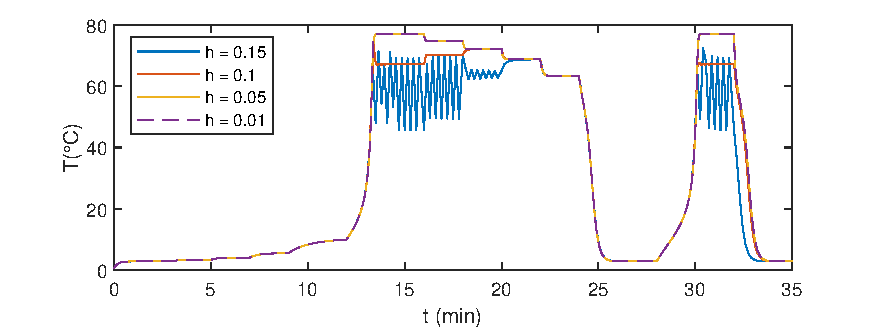
\includegraphics[width=1\linewidth]{images/5/5_5_CSTR_1D.pdf}
        \caption{CSTR 1D problem}
    \end{subfigure}
    \caption{Solution for the CSTR problem using classical Runge-Kutta with fixed step size}
    \label{5_5_3D_1D}
\end{figure}

\subsection{Compare the results from your algorithms with the results you get using some of Matlab's ODE solvers}
As in this part the classical Runge-Kutta with fixed time step size has been the only one implemented, we cannot directly compare to the chosen Matlab solvers (\code{ode45} and \code{ode15s}), as they both use adaptive step size. We'll compare the classical Runge-Kutta in next section, Exercise \ref{6_6}, with its adaptive version.
